\section{Technical Background}

In this chapter, we present background information about technical concepts related to the main topics
of this thesis, which centered around Cross-view Learning with Limited Supervision. We focus on our
background discussion on three topics: multi-view representation learning, relationship quantification, and
self-supervised learning.

The text-to-SQL problem, or NL2SQL, is defined as the following: Given a Natural Language Query (NLQ) on a Relational Database (RDB), produce a SQL query equivalent to the NLQ. Several challenges include ambiguity, schema linking, vocabulary gaps, and user errors.

It has been a holy grail for the database community for over 30 years to translate user queries into SQL. During this section, we will provide a very brief overview of the earlier approaches, especially those that database communities have proposed.

% add image of mindmap here
\begin{figure}[htb]
    \centering
    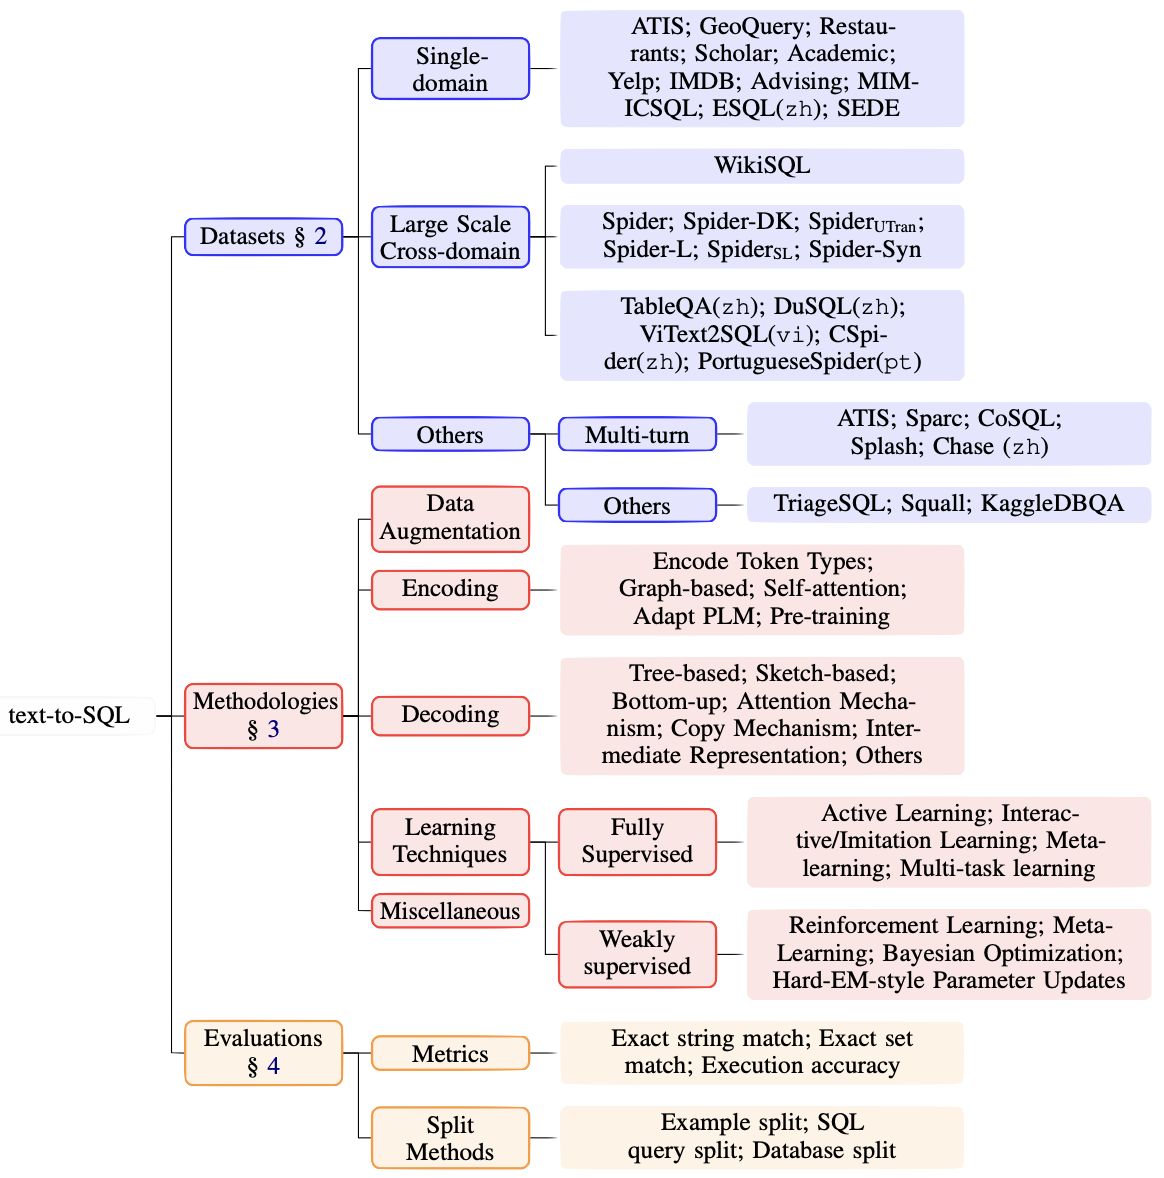
\includegraphics[width=0.6\textwidth]{pics/mindmap.png}
    \caption{Mindmap of the state-of-the-art}
    \label{fig:mindmap}
\end{figure}

\subsection{Early Approaches}

\subsection{Recent Approaches}
